% ==========================================
% BAB IV DESAIN KONSEP SOLUSI
% ==========================================
\chapter{DESAIN KONSEP SOLUSI}
\label{chap:desain-konsep-solusi}
\section{Gambaran Sistem/Kondisi Saat Ini (\textit{As-Is})}

Gambar \ref{gambar: kondisi-as-is} berikut menggambarkan alur deteksi hoaks yang umum terjadi di Indonesia pada praktik sehari-hari. Pengguna membaca sebuah berita, kemudian memeriksa kredibilitasnya melalui situs \textit{fact-checking} seperti MAFINDO/TurnBackHoax. Jika berita tersebut sudah tercatat dalam basis data, statusnya dapat diketahui sebagai hoaks atau bukan. Namun apabila belum tercatat, proses berhenti tanpa kepastian karena tidak ada mekanisme otomatis yang dapat memberikan estimasi lebih lanjut.

\begin{figure}[h!] 
	\centering
  \captionsetup{justification=centering}
    	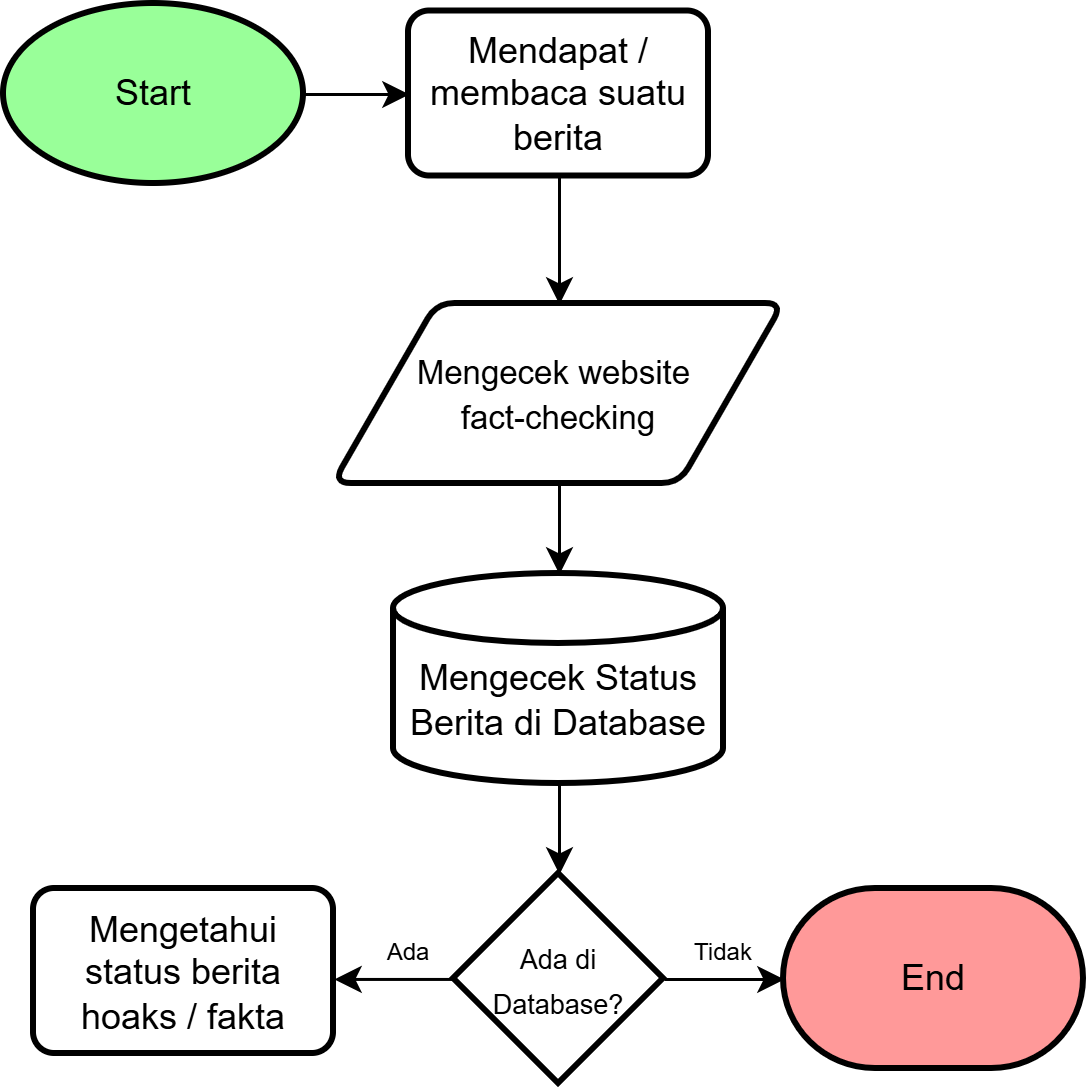
\includegraphics[width=0.7\textwidth]{image/kondisi as-is.png}
	\caption{Kondisi \textit{As-Is} Alur Deteksi Hoaks di Indonesia}
	\label{gambar: kondisi-as-is}
\end{figure}

Penjelasan lebih lanjut mengenai kondisi saat ini menunjukkan adanya kesenjangan antara kebutuhan praktis dan dukungan teknologi yang tersedia. Pada penelitian yang biasa dilakukan, berbagai studi terdahulu telah menerapkan algoritma \textit{machine learning} klasik seperti Naive Bayes, Support Vector Machine, dan Random Forest. Namun setiap penelitian menggunakan \textit{dataset}, tahapan \textit{preprocessing}, dan konfigurasi model yang berbeda-beda sehingga hasilnya sulit dibandingkan secara langsung. Akibatnya, hingga kini belum tersedia \textit{benchmark} terstandarisasi yang dapat memetakan efektivitas relatif ketiga algoritma tersebut dalam konteks berita hoaks berbahasa Indonesia.

Sementara itu, praktik deteksi hoaks di lapangan masih bersifat manual. Proses verifikasi sangat bergantung pada pembaca atau \textit{fact-checker} yang memeriksa kebenaran informasi secara langsung melalui situs pengecekan fakta. Basis data yang tersedia hanya mencakup kasus-kasus yang pernah diperiksa sebelumnya. Berita baru yang belum tercatat tetap harus dinilai secara manual, sehingga proses deteksi tidak bersifat skalabel dan tidak mampu merespons dengan cepat munculnya berita hoaks baru. Selain itu, belum ada sistem pembelajaran mesin yang mempelajari pola teks berita maupun informasi sumber (domain/jenis media) yang dapat memberikan prediksi awal secara otomatis.

Keterbatasan-keterbatasan tersebut menegaskan perlunya desain solusi Tugas Akhir yang mampu menghasilkan \textit{benchmark} algoritma secara terstandar dan menguji secara empiris apakah penambahan fitur sumber dapat meningkatkan kemampuan model dalam mendeteksi hoaks. Bab selanjutnya akan menguraikan rancangan konsep solusi tersebut melalui pembangunan \textit{pipeline} yang terkontrol dan \textit{replicable}.


\section{Desain Konsep Solusi yang Diajukan}

Konsep solusi dalam Tugas Akhir ini berupa \textit{pipeline} eksperimen yang terstandarisasi, yang berfungsi sebagai kerangka evaluasi terukur terhadap tiga algoritma \textit{machine learning} klasik (Naive Bayes, SVM, dan Random Forest) serta dua skenario fitur (\textit{content-only} dan \textit{content+source}). \textit{Pipeline} ini dirancang untuk mereplikasi pola umum penelitian hoaks Indonesia (TF-IDF + ML klasik), sekaligus memperkenalkan blok tambahan berupa pengolahan fitur sumber berita sebagai metadata.

\subsection{Konsep Model Pipeline yang Diusulkan(\textit{To-Be})}

\begin{figure}[h!] 
    \centering
  \captionsetup{justification=centering}
    	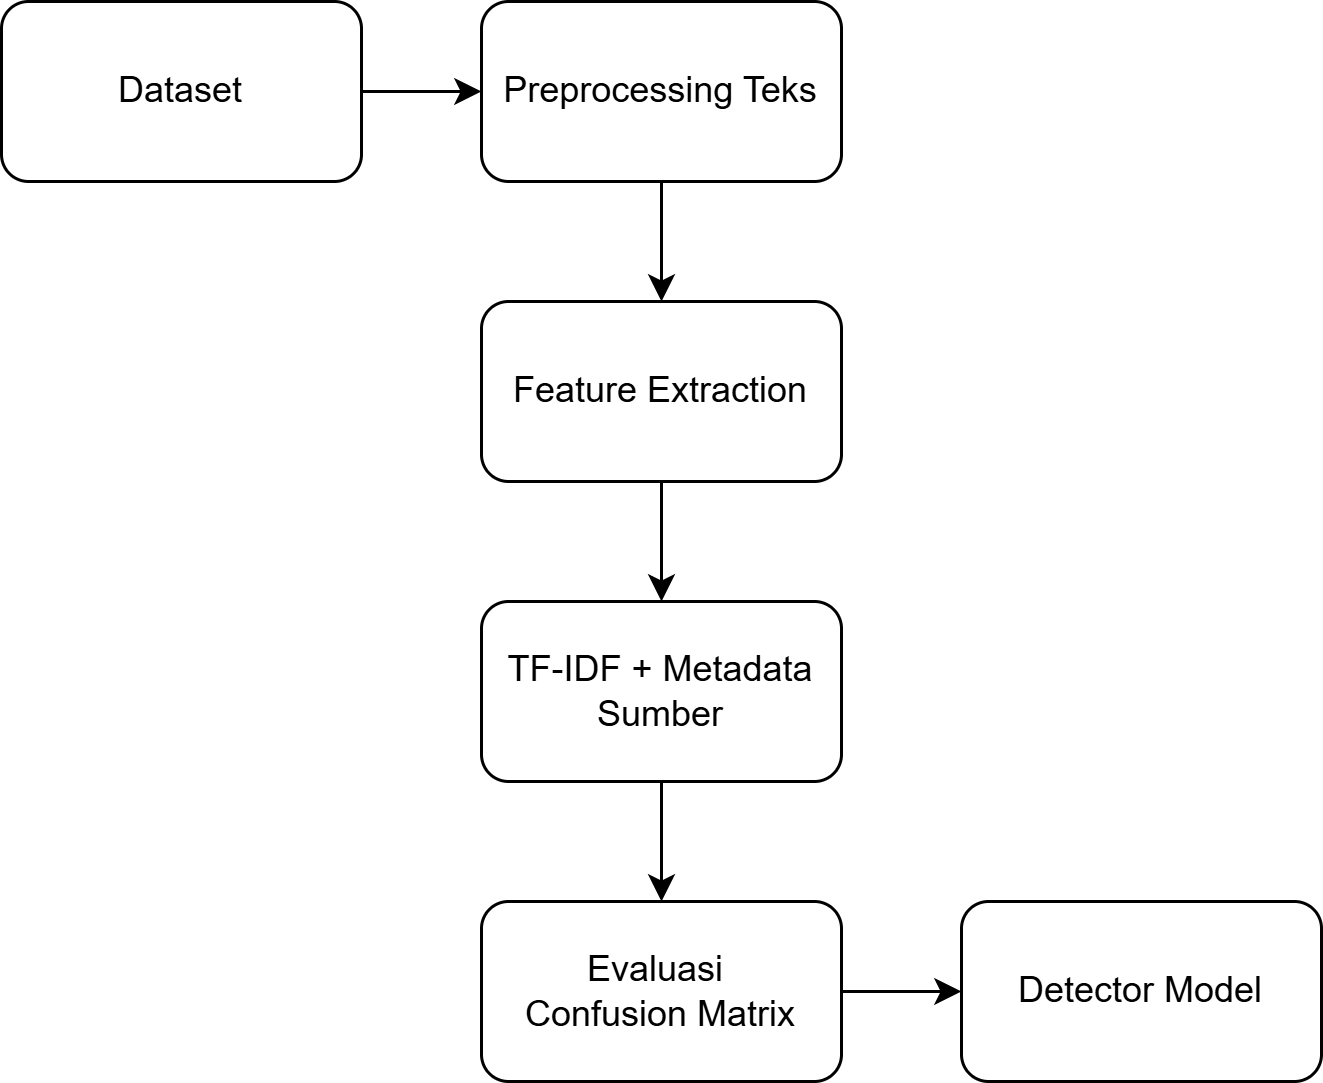
\includegraphics[width=0.9\textwidth]{image/pipeline to-be.png}
    \caption{Kondisi \textit{To-Be} Alur Deteksi Hoaks dengan \textit{Pipeline} yang Diusulkan}
    \label{gambar: pipeline-to-be}
\end{figure}

\textit{Pipeline} yang diusulkan terdiri atas beberapa komponen teknis utama yang saling terhubung secara sistematis:

\begin{enumerate}
\item \textbf{\textit{Dataset}}
    
Komponen pertama mencakup proses pemilihan, pengumpulan, dan pengorganisasian \textit{dataset} berita hoaks dan non-hoaks berbahasa Indonesia. \textit{Dataset} harus memuat tiga elemen penting: 
Pada tahap ini, data disusun dalam format yang konsisten sehingga seluruh sampel dapat melewati \textit{pipeline} secara seragam. Manajemen \textit{dataset} juga mengatur pembagian data ke dalam set pelatihan dan pengujian dengan mekanisme yang konsisten, sehingga hasil evaluasi antar algoritma dapat dibandingkan secara adil.

    \begin{itemize}
        \item Teks berita, yang menjadi objek utama analisis
        \item Label hoaks atau non-hoaks, yang menjadi target pembelajaran
        \item Informasi sumber seperti domain atau jenis media, yang akan digunakan sebagai fitur tambahan pada salah satu skenario.\\
    \end{itemize}



\item \textbf{\textit{Preprocessing}} Teks Bahasa Indonesia

Tahapan \textit{preprocessing} mengikuti praktik terbaik dari penelitian-penelitian yang ada sebelumnya \autocite{pratiwi2022hoax, prasetyo2019evaluation}, meliputi:
    \begin{itemize}
        \item \textbf{Case folding}, yaitu mengubah seluruh teks menjadi huruf kecil untuk menghilangkan variasi kapitalisasi yang tidak membawa makna semantik.

        \item \textbf{Cleaning}, yang mencakup penghapusan angka, simbol, tanda baca tertentu, \textit{hyperlink}, dan elemen non-alfabet lain yang tidak berkontribusi pada makna isi berita.

        \item \textbf{Tokenisasi}, yaitu memecah teks menjadi unit-unit kata, sehingga memungkinkan pembentukan fitur berdasarkan frekuensi dan distribusi kata.

        \item \textbf{Stopword removal}, yaitu menghilangkan kata-kata umum Bahasa Indonesia yang muncul sangat sering tetapi tidak memiliki nilai diskriminatif untuk klasifikasi.

        \item \textbf{Stemming}, yang mengembalikan kata ke bentuk dasarnya untuk menyatukan variasi morfologis, misalnya “menyebarkan”, “disebarkan”, dan “penyebaran” menjadi bentuk dasar “sebar”.

        Proses ini bertujuan menghasilkan representasi teks yang bersih dan dapat diproses lebih lanjut oleh model.\\

    \end{itemize}

    \item \textbf{\textit{Feature Extraction}}
        \begin{enumerate}
            \item \textbf{Fitur Konten (TF-IDF)}
            
            TF-IDF digunakan untuk mengukur tingkat kepentingan suatu kata dalam sebuah dokumen relatif terhadap seluruh korpus. Bobot TF-IDF memastikan bahwa kata-kata yang relevan secara semantik muncul lebih dominan daripada kata umum yang kurang informatif. Representasi ini menghasilkan vektor berdimensi tinggi yang menjadi dasar utama model untuk mengenali pola linguistik khas pada berita hoaks maupun non-hoaks.
            
            \item \textbf{Fitur Sumber (Metadata Domain/Media)}
            
            Informasi mengenai sumber berita, misalnya domain situs atau kategori media, dikodekan ke dalam bentuk numerik melalui teknik seperti one-hot encoding. Representasi ini memetakan setiap sumber ke dalam komponen fitur yang berbeda, memberikan kesempatan bagi model untuk mengidentifikasi kecenderungan atau pola yang berbasis sumber. Penggabungan fitur sumber dilakukan secara modular sehingga dapat dikombinasikan atau dihilangkan sesuai skenario Tugas Akhir.\\
            
            Fitur-fitur ini digunakan untuk membentuk dua skenario percobaan terhadap \textit{pipeline} yang dibangun.\\
        \end{enumerate}

    \item \textbf{Penyusunan Dua Skenario Fitur}
    
        Untuk menguji kontribusi fitur sumber terhadap performa klasifikasi, \textit{pipeline} dirancang dengan dua skenario fitur yang diproses melalui alur identik:
        \begin{itemize}
            \item \textbf{Skenario 1 : \textit{Content-only }}
            
            Menggunakan hanya fitur TF-IDF. Skenario ini berfungsi sebagai baseline dan merepresentasikan pendekatan penelitian terdahulu yang umumnya bergantung pada konten teks saja.

            \item \textbf{Skenario 2 : \textit{Content + Source}} (menggabungkan TF-IDF dengan fitur sumber.)
            
            Menggabungkan fitur TF-IDF dengan fitur sumber hasil encoding. Skenario ini memungkinkan evaluasi empiris mengenai apakah penambahan informasi sumber memberikan peningkatan performa atau tidak.\\

        \end{itemize}
        
        Kedua skenario ini disusun untuk memastikan bahwa efek penambahan metadata dapat dinilai secara objektif karena seluruh elemen \textit{pipeline} selain fitur tetap sama.\\
    
    \item \textbf{Pelatihan Model ML Klasik}
    
    Ketiga algoritma (Naive Bayes, SVM, Random Forest) dilatih pada kedua skenario fitur. Tujuannya adalah membentuk \textit{benchmark} performa yang konsisten dalam satu \textit{pipeline} terkontrol.

    \item \textbf{Evaluasi Performa Model}
    
    Model dievaluasi menggunakan metrik standar klasifikasi \textit{Confusion Matrix}: \textit{accuracy, precision, recall, F1-score}.

    Metrik ini dipilih karena telah digunakan secara konsisten dalam penelitian deteksi hoaks Indonesia \autocite{triyono2023indonesian, safira2023comparative}.

    \item \textbf{\textit{Output Benchmark} dan Analisis Pengaruh Fitur Sumber}

    Hasil dari kedua skenario dibandingkan untuk menilai apakah penambahan fitur sumber meningkatkan performa model secara signifikan. \\

\end{enumerate}

\textit{Pipeline} ini menjadi kerangka dasar untuk eksperimen yang \textit{replicable} dan dapat memberikan pemahaman lebih terukur mengenai efektivitas relatif NB, SVM, dan RF, sekaligus kontribusi fitur sumber.

\subsection{Kondisi \textit{To-Be}}

\begin{figure}[H]
    \centering
  \captionsetup{justification=centering}
    	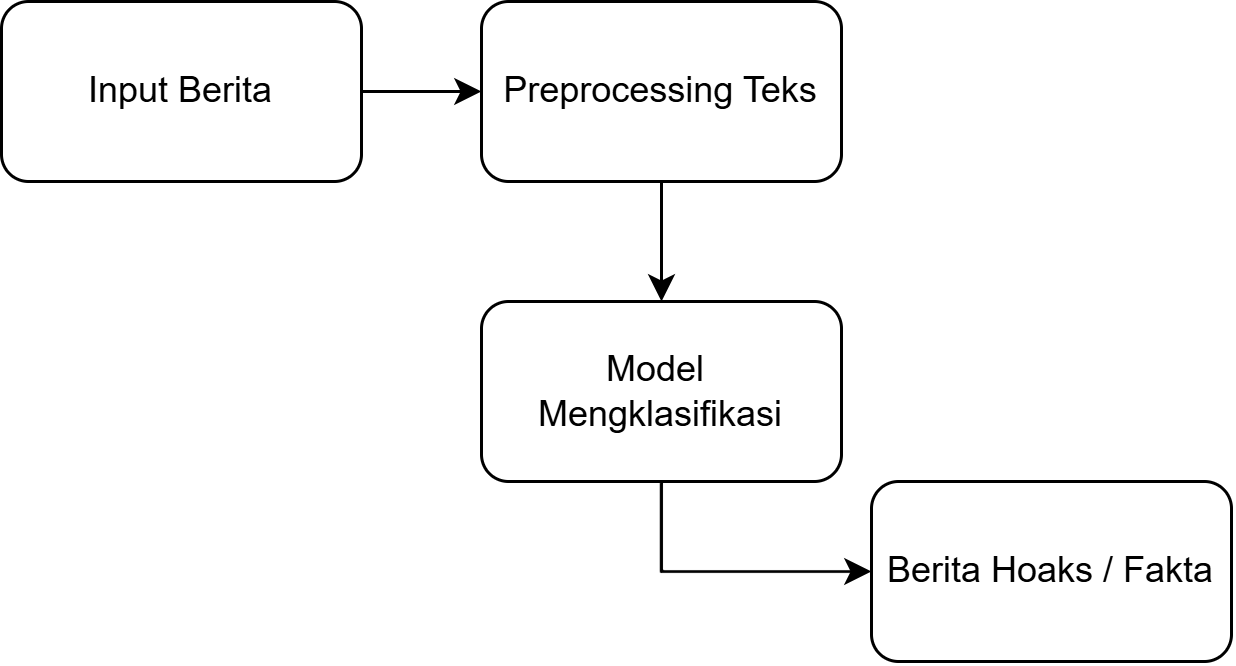
\includegraphics[width=0.9\textwidth]{image/kondisi to-be.png}
    \caption{Kondisi \textit{To-Be} Alur Deteksi Hoaks di Indonesia}
    \label{gambar: kondisi-to-be}
\end{figure}

Alur pada Gambar \ref{gambar: kondisi-to-be} menunjukkan bagaimana model yang dihasilkan dari \textit{pipelin}e Tugas Akhir ini dapat digunakan untuk memproses berita baru. Proses dimulai ketika pengguna memasukkan teks berita yang ingin diperiksa, disertai informasi sumber apabila tersedia. Berita tersebut kemudian menjalani tahapan \textit{preprocessing} yang sama dengan tahapan saat pelatihan, sehingga konsistensi struktur data tetap terjaga dan model menerima masukan dalam format yang sesuai.

Teks yang telah melalui \textit{preprocessing} diubah menjadi representasi numerik menggunakan TF-IDF vectorizer dan encoder fitur sumber yang sudah tertanam di dalam model. Dengan demikian, seluruh berita baru diproyeksikan ke dalam ruang fitur yang sama seperti data pelatihan. Setelah representasi fitur terbentuk, model melakukan inferensi dan menghasilkan keluaran berupa prediksi kelas hoaks atau fakta. Proses ini menggambarkan bagaimana model dapat digunakan sebagai mekanisme penyaringan awal sebelum dilakukan verifikasi manual yang lebih mendalam.

Perlu ditegaskan bahwa alur penggunaan ini merupakan ilustrasi potensi pemanfaatan model di masa mendatang. Pada tahap tugas akhir, fokus utama penggunaan model masih berada pada konteks eksperimen dan evaluasi performa dalam lingkungan yang terkontrol.


\section{Perbandingan Kondisi As-Is dan Konsep Solusi (\textit{To-Be})}
Solusi yang diusulkan memberikan penyelesaian langsung terhadap berbagai keterbatasan kondisi saat ini. Tabel berikut merangkum perbandingan tersebut. \\

\input table/tabel-perbandingan-kondisi.tex

Tabel \ref{tbl:perbandingan-pendekatan} merangkum perbedaan antara kondisi saat ini dan konsep solusi yang diusulkan melalui \textit{pipeline} Tugas Akhir ini. Kondisi saat ini ditandai oleh penelitian terdahulu yang menggunakan algoritma \textit{machine learning} klasik tetapi dengan konfigurasi, \textit{dataset}, dan \textit{preprocessing} yang berbeda-beda, sehingga hasilnya sulit dibandingkan secara langsung. Di sisi praktik lapangan, deteksi hoaks masih sangat bergantung pada verifikasi manual serta basis data yang terbatas pada kasus yang sudah pernah diperiksa, tanpa adanya model prediktif yang dapat memberikan estimasi awal untuk berita baru.

Konsep solusi yang diusulkan menyediakan kerangka eksperimen yang terstandarisasi melalui \textit{pipeline} yang menerapkan \textit{dataset} konsisten, \textit{preprocessing} yang seragam, dua skenario fitur yang terkontrol, serta evaluasi kinerja menggunakan metrik yang sama untuk semua model. Pendekatan ini menghasilkan \textit{benchmark} yang dapat dibandingkan secara adil antar algoritma serta memungkinkan analisis empiris mengenai pengaruh penambahan fitur sumber terhadap performa deteksi.

Keberadaan detector model dan alur penggunaan pada Gambar \ref{gambar: kondisi-to-be} menunjukkan bahwa \textit{pipelin}e yang dirancang tidak hanya berfungsi sebagai alat evaluasi, tetapi juga membuka peluang pengembangan model sebagai komponen \textit{screening} otomatis bagi berita baru di masa mendatang. Dengan demikian, konsep solusi ini menjembatani kesenjangan antara kebutuhan praktis deteksi hoaks dan fragmentasi hasil penelitian sebelumnya.